\documentclass{article}
\usepackage[utf8]{inputenc}
\title{Sentiment Classification based on LSTM}
\author{
  Chengzhen Wang\\
  \texttt{3401-7634-21}\\
  \texttt{chengzhw@usc.edu}
  \and
  Guannan Meng\\
  \texttt{1586-2580-67}\\
  \texttt{guannanm@usc.edu}
  \and
  Qixuan Wang\\
  \texttt{5497-0747-37}\\
  \texttt{qixuanwa@usc.edu}
}
\date{April 2016}

\usepackage{natbib}
\usepackage{amsmath, amsthm, amssymb, amsfonts}
\usepackage{graphicx}

\begin{document}

\maketitle

\section{Introduction}
The development of web technologies leads to the explosion of web opinion data about products, services, public events and many other entities. These thousands of data can be used for public opinion analysis. For example, after reading product reviews from other customers, people can make wiser decisions that whether to buy some products or not. Although the valuable opinion data are rapidly increasing day and night, the arduous workload for reading and analyzing large scale data is impossible for individuals. It brings a pressing need for building the system which can perform sentiment classification (or opinion mining) job automatically.


To solve this problem, researchers have proposed many applications such as opinion summarization, opinion ranking, and opinion retrieval etc. \cite{liu2012sentiment}\cite{pang2008opinion}. Mainstream applications treat this problem as a classification problem which can be solved by heuristic models or machine learning models. Most of these models assign a sentiment polarity (e.g., “positive” or “negative” or “neutral”) to the text.


However, most of the existing models only focus on a specific domain or similar domains which cannot be adapted to other domains. Our goal is to propose a general model which can be trained one time with large scale corpus consisting of texts from multiple domains and utilized in any domains directly. Inspired by T. Mikolov's RNNLM\cite{mikolov2011rnnlm}, we plan to use a RNN (Recurrent Neural Network) model to train a language model with massive amounts of Japanese customer reviews from multiple domains. Then we train and test our sentiment classifier with the trained words embedding (distributed representation) from the language model. In this research, we employed the Long short-term memory (LSTM) RNN model \cite{hochreiter1997long}\cite{graves2012supervised} to train our language model and word embeddings.

The experiments show that our LSTM-based language model provide great word embeddings and eventually get the best performance in the sentiment classification evaluation compare to other baseline methods.
% \begin{figure}[h!]
% \centering
% 
\includegraphics[scale=1.7]{universe.jpg}
% \caption{The Universe}
% \label{fig:univerise}
% \end{figure}

\section{Method}
\subsection{Materials}

\subsection{Procedure}
After gathering the corpus and dealing the preprocessing, we can now start to building the language model and get the word embeddings. Since the recurrent neural network is proved to be success in the building of language model for long text\cite{mikolov2011rnnlm}, we choose long short-term memory (LSTM) as the core module of our framework to build the language model. LSTM is a modified RNN model which is designed to overcome some defacts of the RNN such as the \textit{vanishing gradient} and \textit{exploding gradients}. Therefore, the \textit{memory cell} is introduced to the LSTM node. As shown in figure \ref{fig:lstmnode}, such memory cell contains an input gate, a memory cell, a forget gate, and an output gate.
\begin{figure}[htb]
\centering
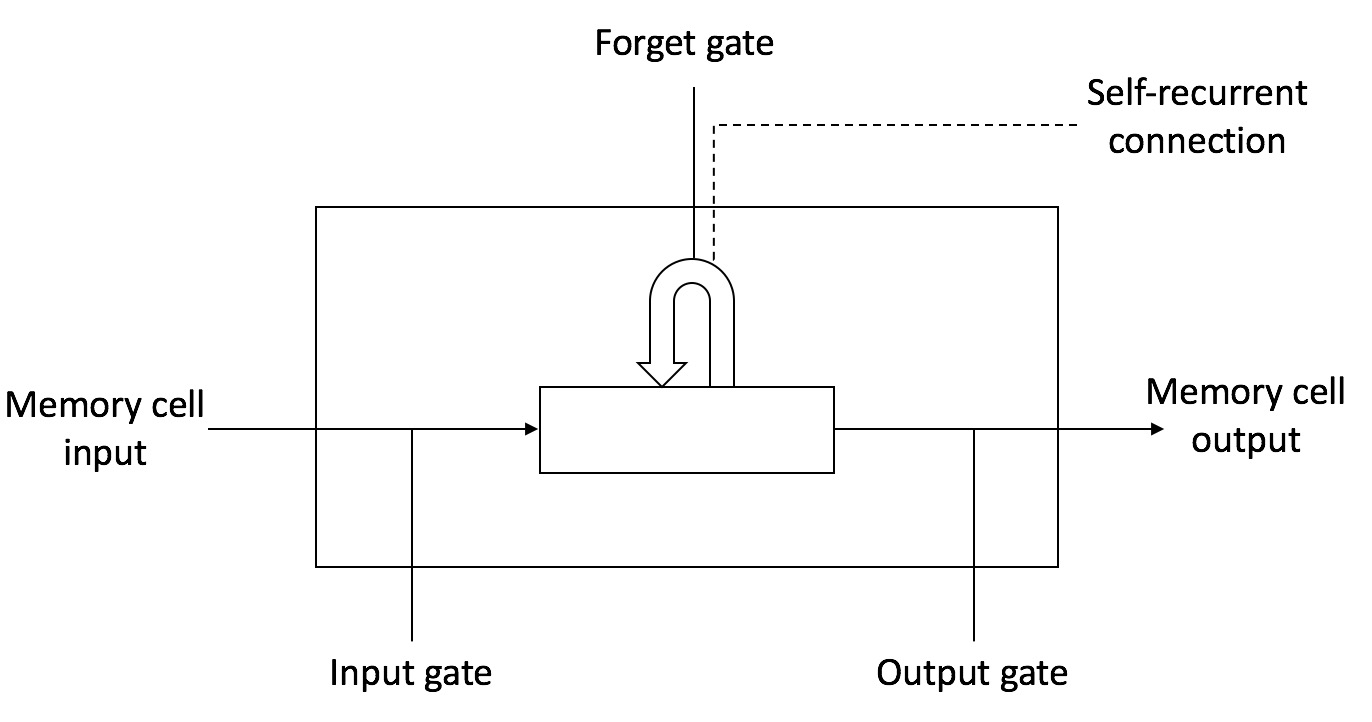
\includegraphics[scale=0.2]{LSTMNODE.png}
\caption{Recurrent Neural Network Language Model.}
\label{fig:lstmnode}
\end{figure}

To update memory cells for every token $w_{t}$, the standard LSTM model adopted following notations and equations:
\begin{itemize}
  \item $w_{t}$ is the $t^{th}$ token input
  \item $W$, $U$, and $V$ are LSTM weights
  \item $b$ are bias vectors
  \item $i_{t}$ is the $t^{th}$ input gate
  \item $\overline {C}_{t}$ is the $t^{th}$ candidate value for the states of the memory cell
  \item $f_{t}$ is the actication of forget gates gate
  \item $C_{t}$ is the $t^{th}$ new candidate state for the memory cell
  \item $o_{t}$ is the value of output gate and $h_{t}$ is the output of the LSTM node
\end{itemize}


$$i_{t}=\sigma(W_{i}w_{t}+U_{i}h_{t-1}+b_{i})$$
$$\overline {C}_{t}=\tanh(W_{c}w_{t}+U_{c}h_{t-1}+b_{c})$$
$$f_{t}=\sigma(W_{f}w_{t}+U_{f}h_{t-1}+b_{f})$$
$$C_{t}=i_{t}\ast \overline {C}_{t} + f_{t} \ast C_{t-1}$$
$$o_{t}=\sigma(W_{o}w_{t}+U_{o}h_{t-1}+V_{o}C_{t}+b_{o})$$
$$h_{t}=o_{t} \ast \tanh(C_{t})$$
 
In order to build appropriate language model that can provide high quality word embeddings for the sentiment classification, the model we adopted add a mean pooling layer which will count the mean vector of the output vector $h_{i}$ of each token $i$ in one customer review. Then, the mean vector \textit{h} and the corresponding sentiment polarity label (positive:1 or negative:0) is used as the input of a logistic regression layer which help to train the weights of LSTM node through backpropagation process. The architecture of the model is shown in figure \ref{fig:lstmmodel}. We implement this model by following this tutorial \cite{lstmtutorial} and using \textit{Theano}\footnote{http://deeplearning.net/software/theano/}, which is a python library for implementing deeplearning algorithms.
\begin{figure}[htb]
\centering
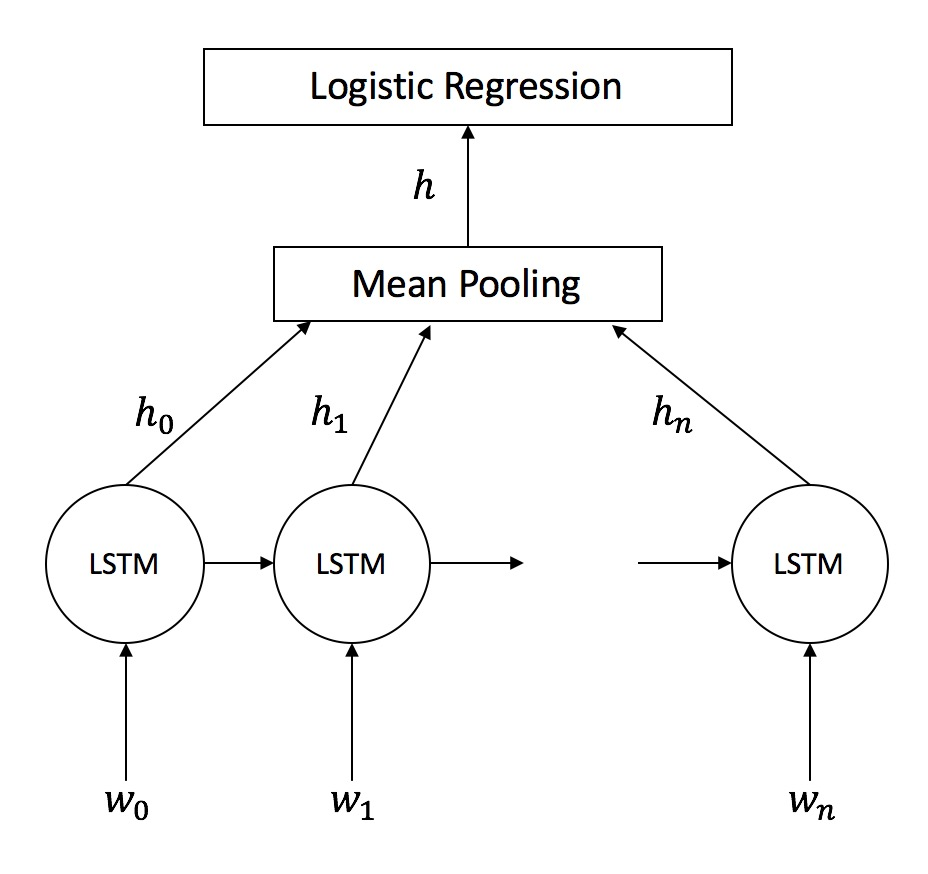
\includegraphics[scale=0.2]{LSTMMODEL.png}
\caption{Recurrent Neural Network Language Model.}
\label{fig:lstmmodel}
\end{figure}


To train our model, we firstly convert the Japanese corpus to "index" representation. Which means use correspoinding index from the vocabulary replace each real japanese word. So that a review will be translated to a list of integers. For each word, the index will firstly represented by a random $d$ dimensional vector as its initial distributed representation. The $d$ is set by ourselves which represent the dimension of the word embeddings we want to trained. Eventually, after the model converged, we fetch the word embeddings from the trained weight. The word embeddings will be a $\left| V\right| \ast d$ matrix that each vector $v_{i}$ of row $i$ is the distributed representation of $i^{th}$ word in the vocabulary. The $\left| V\right|$ is the size of the vocabulary. Finally, the word embeddings will be used to build the sample vector for training the sentiment classifier. We will discuss the training steps and the evaluation of the sentiment classification in next section.


\subsection{Evaluation}

\subsubsection{RNNLM}

\begin{figure}[htb]
\centering
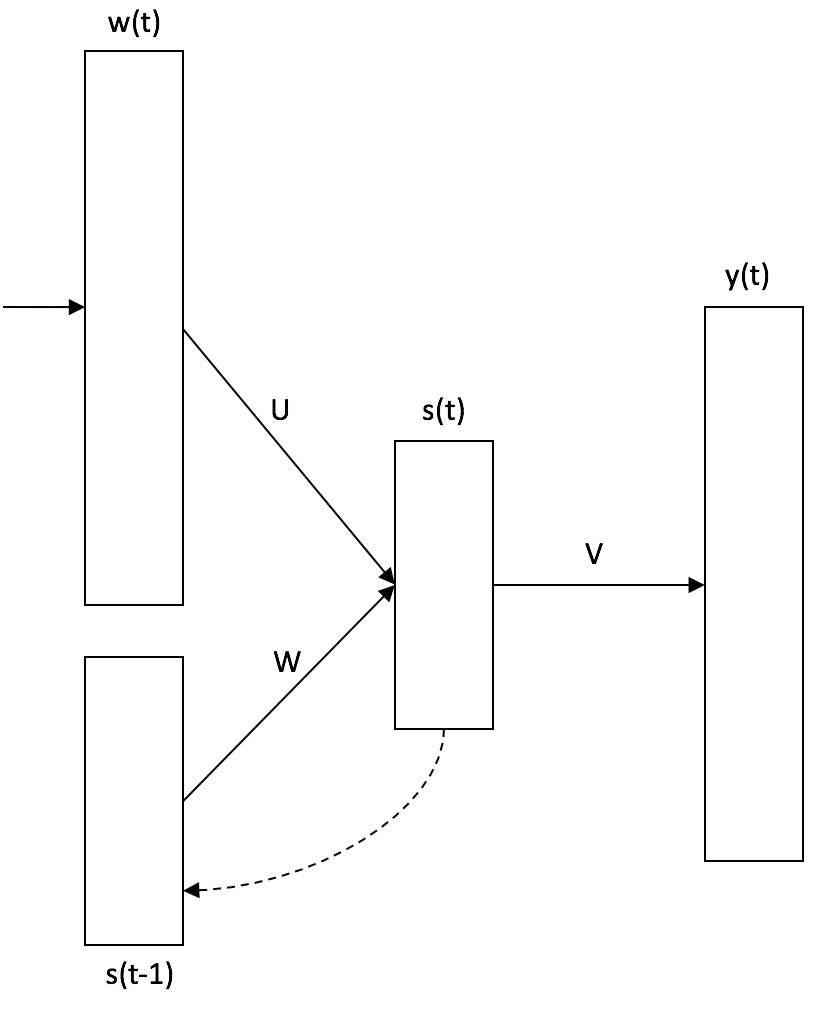
\includegraphics[scale=0.2]{RNNLM.png}
\caption{Recurrent Neural Network Language Model.}
\label{fig:rnnlm}
\end{figure}

\section{Results}


\section{Discussion}



\bibliographystyle{plain}
\bibliography{references}

\section{Division of Labor}


\section{Word Count}


\end{document}
